\documentclass[12pt,letterpaper]{article}
\usepackage{graphicx,textcomp}
\usepackage{natbib}
\usepackage{setspace}
\usepackage{fullpage}
\usepackage{color}
\usepackage[reqno]{amsmath}
\usepackage{amsthm}
\usepackage{fancyvrb}
\usepackage{amssymb,enumerate}
\usepackage[all]{xy}
\usepackage{endnotes}
\usepackage{lscape}
\newtheorem{com}{Comment}
\usepackage{float}
\usepackage{hyperref}
\newtheorem{lem} {Lemma}
\newtheorem{prop}{Proposition}
\newtheorem{thm}{Theorem}
\newtheorem{defn}{Definition}
\newtheorem{cor}{Corollary}
\newtheorem{obs}{Observation}
\usepackage[compact]{titlesec}
\usepackage{dcolumn}
\usepackage{tikz}
\usetikzlibrary{arrows}
\usepackage{multirow}
\usepackage{xcolor}
\newcolumntype{.}{D{.}{.}{-1}}
\newcolumntype{d}[1]{D{.}{.}{#1}}
\definecolor{light-gray}{gray}{0.65}
\usepackage{url}
\usepackage{listings}
\usepackage{color}

\definecolor{codedarkred}{rgb}{0.55,0,0}
\definecolor{codedarkblue}{rgb}{0,0,0.55}
\definecolor{codegray}{rgb}{0.5,0.5,0.5}
\definecolor{backcolour}{rgb}{0.95,0.95,0.92}

\lstdefinestyle{mystyle}{
	backgroundcolor=\color{backcolour},   
	basicstyle=\footnotesize\color{codedarkblue},
	commentstyle=\color{codedarkred},
	keywordstyle=\color{codedarkred},
	numberstyle=\tiny\color{codegray},
	stringstyle=\color{codedarkred},
	breakatwhitespace=false,         
	breaklines=true,                 
	captionpos=b,                    
	keepspaces=true,                 
	numbers=left,                    
	numbersep=5pt,                  
	showspaces=false,                
	showstringspaces=false,
	showtabs=false,                  
	tabsize=2
}
\lstset{style=mystyle}
\newcommand{\Sref}[1]{Section~\ref{#1}}
\newtheorem{hyp}{Hypothesis}

\title{Problem Set 3}
\date{Due: November 12, 2026\\[0.5em]Emilia Lupi}
\author{Applied Stats/Quant Methods 1}


\begin{document}
	\maketitle
	\section*{Instructions}
	\begin{itemize}
		\item Please show your work! You may lose points by simply writing in the answer. If the problem requires you to execute commands in \texttt{R}, please include the code you used to get your answers. Please also include the \texttt{.R} file that contains your code. If you are not sure if work needs to be shown for a particular problem, please ask.
		\item Your homework should be submitted electronically on GitHub.
		\item This problem set is due before 23:59 on Thursday November 12, 2026. No late assignments will be accepted.
		
	\end{itemize}
	
	\vspace{.25cm}
	
	\noindent In this problem set, you will run several regressions and create an add variable plot (see the lecture slides) in \texttt{R} using the \texttt{incumbents\_subset.csv} dataset. Include all of your code.
	
	\vspace{.5cm}
	\section*{Question 1}
	\vspace{.25cm}
	\noindent We are interested in knowing how the difference in campaign spending between incumbent and challenger affects the incumbent's vote share. 
	\begin{enumerate}
		\item Run a regression where the outcome variable is \texttt{voteshare} and the explanatory variable is \texttt{difflog}.
		
		\noindent To run the regression, I used the \texttt{lm()} function in \texttt{R}, with \texttt{voteshare} as the outcome variable and \texttt{difflog} as the explanatory variable. The results are reported in Table~\ref{tab:regression_q1}.
		
		\lstinputlisting[language=R, firstline=51, lastline=51]{PS03_answersEL.R}
		
		
\begin{table}[H] \centering 
  \caption{Regression of incumbent's vote share on difference in spending} 
  \label{tab:regression_q1} 
\begin{tabular}{@{\extracolsep{5pt}}lc} 
\\[-1.8ex]\hline 
\hline \\[-1.8ex] 
 & \multicolumn{1}{c}{\textit{Dependent variable:}} \\ 
\cline{2-2} 
\\[-1.8ex] & Incumbent's vote share (voteshare) \\ 
\hline \\[-1.8ex] 
 Difference in spending (difflog) & 0.042$^{***}$ \\ 
  & (0.001) \\ 
  & \\ 
 Constant & 0.579$^{***}$ \\ 
  & (0.002) \\ 
  & \\ 
\hline \\[-1.8ex] 
Observations & 3,193 \\ 
R$^{2}$ & 0.367 \\ 
Adjusted R$^{2}$ & 0.367 \\ 
Residual Std. Error & 0.079 (df = 3191) \\ 
F Statistic & 1,852.791$^{***}$ (df = 1; 3191) \\ 
\hline 
\hline \\[-1.8ex] 
\textit{Note:}  & \multicolumn{1}{r}{$^{*}$p$<$0.1; $^{**}$p$<$0.05; $^{***}$p$<$0.01} \\ 
\end{tabular} 
\end{table}  

		
		\noindent The intercept (0.579) is the predicted vote share of the incumbent when \texttt{difflog} is 0, that is, when the incumbent and the challenger spend the same amount. In this case the incumbent is predicted to get about 57.9\% of the vote. The slope (0.042) means that a one unit increase in \texttt{difflog} is associated with an increase of about 0.042 in the incumbent's vote share. The p-value of the slope is below 0.01, so we reject the null hypothesis that $\beta_1 = 0$: the relationship is statistically significant. The $R^2$ shows that \texttt{difflog} explains about 36.7\% of the variation in \texttt{voteshare}.
		
		\item Make a scatterplot of the two variables and add the regression line.
		
		\lstinputlisting[language=R, firstline=63, lastline=68]{PS03_answersEL.R}
		
		\begin{figure}[H]
			\centering
			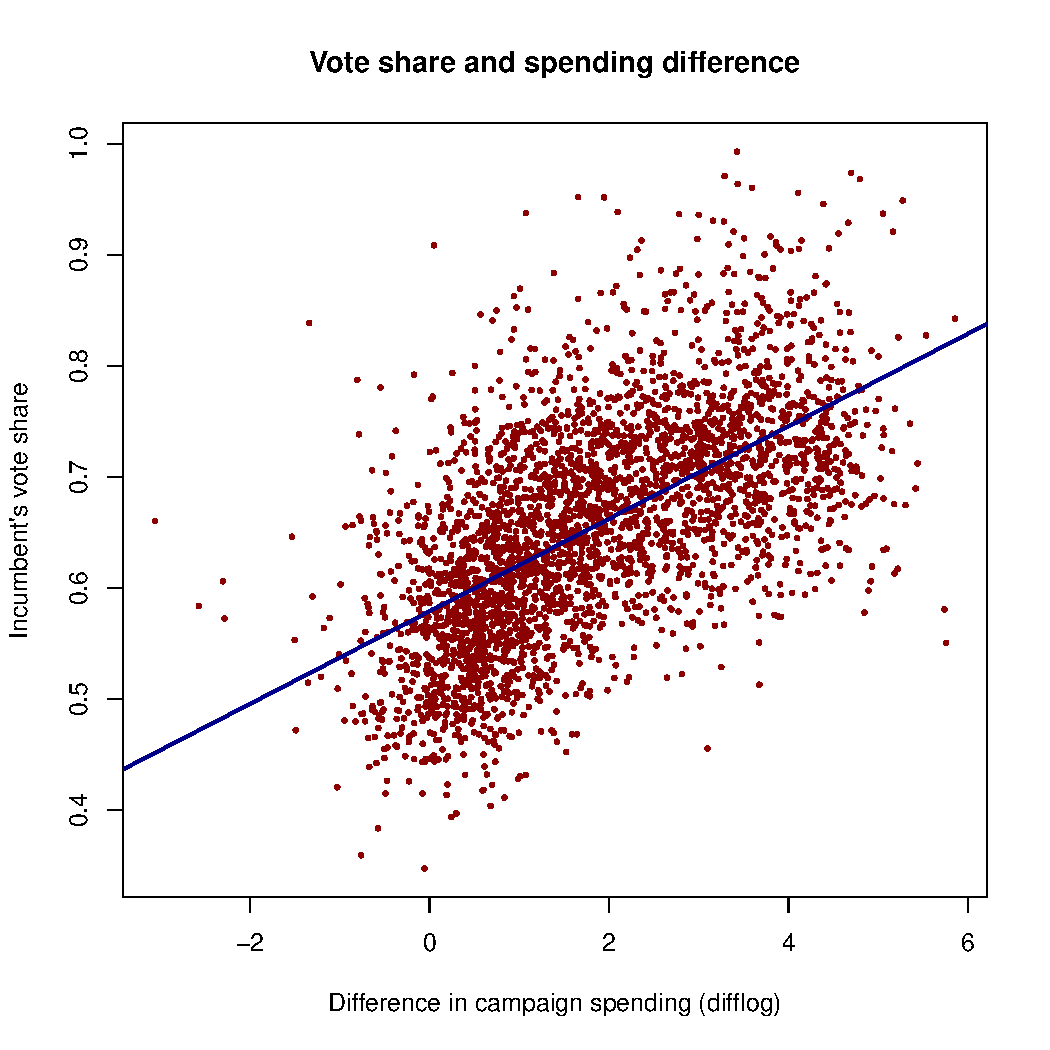
\includegraphics[width=0.7\textwidth]{plot_q1.pdf}
			\caption{Scatterplot of \texttt{voteshare} and \texttt{difflog} with the regression line}
		\end{figure}
		
		\noindent The scatterplot shows a clear positive relationship between the difference in campaign spending and the incumbent's vote share: when the incumbent spends more than the challenger, the incumbent tends to get a higher vote share.
		
		\item Save the residuals of the model in a separate object.
		
		\lstinputlisting[language=R, firstline=72, lastline=72]{PS03_answersEL.R}
		
		
\begin{table}[H] \centering 
  \caption{Summary of the residuals of Question 1 (resid\_1)} 
  \label{tab:resid_q1} 
\begin{tabular}{@{\extracolsep{5pt}} cccccc} 
\\[-1.8ex]\hline 
\hline \\[-1.8ex] 
Min. & 1st Qu. & Median & Mean & 3rd Qu. & Max. \\ 
\hline \\[-1.8ex] 
$$-$0.2683$ & $$-$0.0535$ & $$-$0.0038$ & $$-$0$ & $0.0478$ & $0.3275$ \\ 
\hline \\[-1.8ex] 
\end{tabular} 
\end{table}  

		
		\noindent Each residual is the difference between the observed vote share and the vote share predicted by the model, $\hat{\varepsilon}_i = y_i - \hat{y}_i$. They show the part of \texttt{voteshare} that is not explained by \texttt{difflog}. Their mean is 0, as always in OLS with an intercept. This means that the positive and negative residuals cancel out exactly, so their sum and their average are both 0
		
		\item Write the prediction equation.
		
		\[
		\widehat{\texttt{voteshare}}_i = 0.579 + 0.042 \times \texttt{difflog}_i
		\]
	\end{enumerate}
	
	\section*{Question 2}
	\noindent We are interested in knowing how the difference between incumbent and challenger's spending and the vote share of the presidential candidate of the incumbent's party are related.	\vspace{.25cm}
	\begin{enumerate}
		\item Run a regression where the outcome variable is \texttt{presvote} and the explanatory variable is \texttt{difflog}.
		
		\noindent To run the regression, I used the \texttt{lm()} function in \texttt{R}, with \texttt{presvote} as the outcome variable and \texttt{difflog} as the explanatory variable. The results are reported in Table~\ref{tab:regression_q2}.
		
		\lstinputlisting[language=R, firstline=93, lastline=93]{PS03_answersEL.R}
		
		
\begin{table}[H] \centering 
  \caption{Regression of presidential vote share on difference in spending} 
  \label{tab:regression_q2} 
\begin{tabular}{@{\extracolsep{5pt}}lc} 
\\[-1.8ex]\hline 
\hline \\[-1.8ex] 
 & \multicolumn{1}{c}{\textit{Dependent variable:}} \\ 
\cline{2-2} 
\\[-1.8ex] & Vote share of the president's party (presvote) \\ 
\hline \\[-1.8ex] 
 Difference in spending (difflog) & 0.024$^{***}$ \\ 
  & (0.001) \\ 
  & \\ 
 Constant & 0.508$^{***}$ \\ 
  & (0.003) \\ 
  & \\ 
\hline \\[-1.8ex] 
Observations & 3,193 \\ 
R$^{2}$ & 0.088 \\ 
Adjusted R$^{2}$ & 0.088 \\ 
Residual Std. Error & 0.110 (df = 3191) \\ 
F Statistic & 307.715$^{***}$ (df = 1; 3191) \\ 
\hline 
\hline \\[-1.8ex] 
\textit{Note:}  & \multicolumn{1}{r}{$^{*}$p$<$0.1; $^{**}$p$<$0.05; $^{***}$p$<$0.01} \\ 
\end{tabular} 
\end{table}  

		
		\noindent When the two candidates spend the same amount (\texttt{difflog} $= 0$), the predicted vote share of the presidential candidate of the incumbent's party is about 50.8\% (intercept). A one unit increase in \texttt{difflog} is associated with an increase of about 0.024 in \texttt{presvote}. The slope is statistically significant (p-value $< 0.001$). However, the $R^2$ is 0.088, which means that \texttt{difflog} explains only about 8.8\% of the variation in \texttt{presvote}, so most of the differences in the presidential vote share across districts depend on other factors.
		
		\item Make a scatterplot of the two variables and add the regression line.
		
		\lstinputlisting[language=R, firstline=105, lastline=110]{PS03_answersEL.R}
		
		\begin{figure}[H]
			\centering
			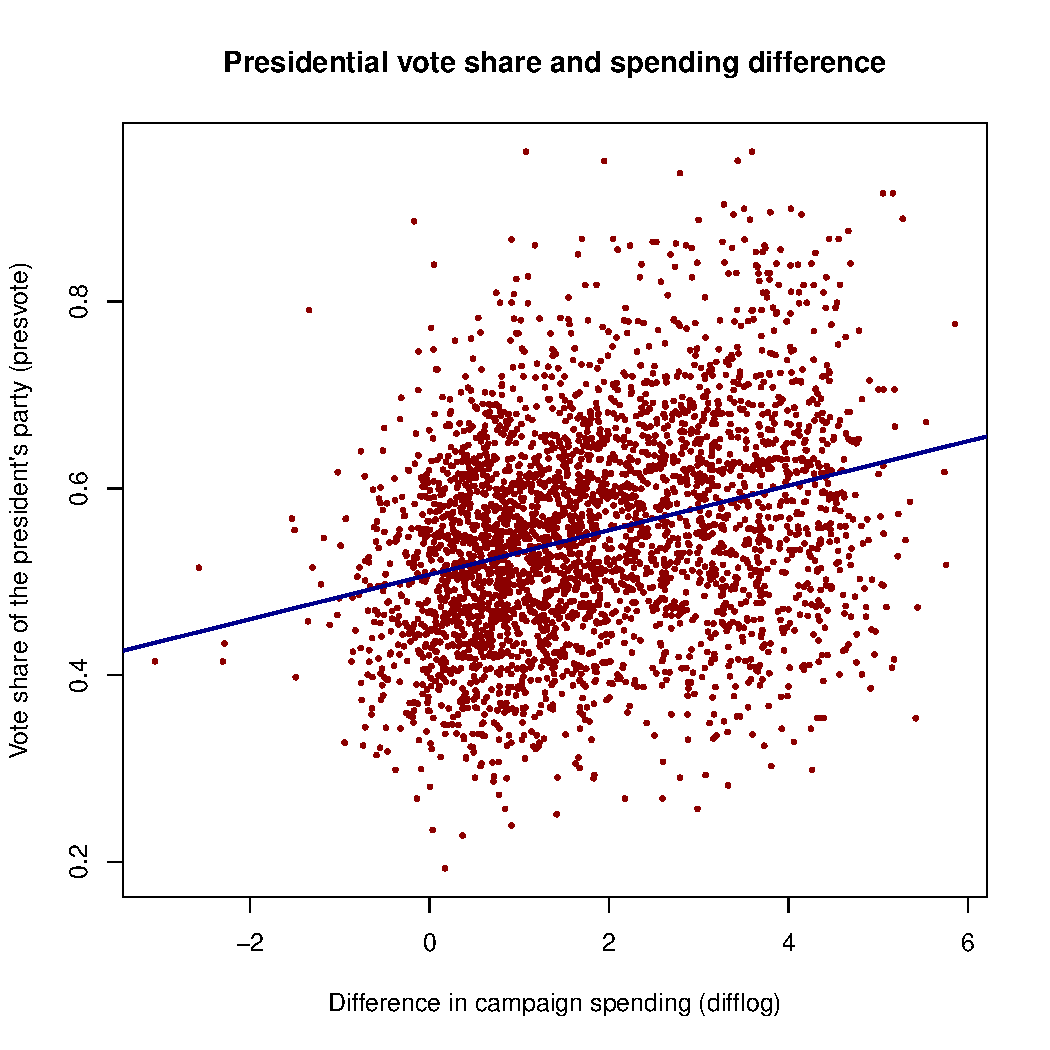
\includegraphics[width=0.7\textwidth]{plot_q2.pdf}
			\caption{Scatterplot of \texttt{presvote} and \texttt{difflog} with the regression line}
		\end{figure}
		
		\noindent The scatterplot shows a positive relationship between the difference in campaign spending and the vote share of the presidential candidate of the incumbent's party, since the regression line goes upward. However, the line is quite flat compared to how widely the points are spread, so knowing the spending difference in a district does not help much to predict the presidential vote share there, which is consistent with the low $R^2$.
		
		\item Save the residuals of the model in a separate object.
		
		\lstinputlisting[language=R, firstline=114, lastline=114]{PS03_answersEL.R}
		
		
\begin{table}[H] \centering 
  \caption{Summary of the residuals of Question 2 (resid\_2)} 
  \label{tab:resid_q2} 
\begin{tabular}{@{\extracolsep{5pt}} cccccc} 
\\[-1.8ex]\hline 
\hline \\[-1.8ex] 
Min. & 1st Qu. & Median & Mean & 3rd Qu. & Max. \\ 
\hline \\[-1.8ex] 
$$-$0.3220$ & $$-$0.0741$ & $$-$0.0010$ & $0$ & $0.0715$ & $0.4274$ \\ 
\hline \\[-1.8ex] 
\end{tabular} 
\end{table}  

		
		\noindent These residuals show the part of \texttt{presvote} that is not explained by \texttt{difflog}.
		
		\item Write the prediction equation.
		
		\[
		\widehat{\texttt{presvote}}_i = 0.508 + 0.024 \times \texttt{difflog}_i
		\]
	\end{enumerate}
	
	\section*{Question 3}
	
	\noindent We are interested in knowing how the vote share of the presidential candidate of the incumbent's party is associated with the incumbent's electoral success.
	\vspace{.25cm}
	\begin{enumerate}
		\item Run a regression where the outcome variable is \texttt{voteshare} and the explanatory variable is \texttt{presvote}.
		
		\noindent To run the regression, I used the \texttt{lm()} function in \texttt{R}, with \texttt{voteshare} as the outcome variable and \texttt{presvote} as the explanatory variable. The results are reported in Table~\ref{tab:regression_q3}.
		
		\lstinputlisting[language=R, firstline=135, lastline=135]{PS03_answersEL.R}
		
		
\begin{table}[H] \centering 
  \caption{Regression of incumbent's vote share on presidential vote share} 
  \label{tab:regression_q3} 
\begin{tabular}{@{\extracolsep{5pt}}lc} 
\\[-1.8ex]\hline 
\hline \\[-1.8ex] 
 & \multicolumn{1}{c}{\textit{Dependent variable:}} \\ 
\cline{2-2} 
\\[-1.8ex] & Incumbent's vote share (voteshare) \\ 
\hline \\[-1.8ex] 
 Vote share of the president's party (presvote) & 0.388$^{***}$ \\ 
  & (0.013) \\ 
  & \\ 
 Constant & 0.441$^{***}$ \\ 
  & (0.008) \\ 
  & \\ 
\hline \\[-1.8ex] 
Observations & 3,193 \\ 
R$^{2}$ & 0.206 \\ 
Adjusted R$^{2}$ & 0.206 \\ 
Residual Std. Error & 0.088 (df = 3191) \\ 
F Statistic & 826.950$^{***}$ (df = 1; 3191) \\ 
\hline 
\hline \\[-1.8ex] 
\textit{Note:}  & \multicolumn{1}{r}{$^{*}$p$<$0.1; $^{**}$p$<$0.05; $^{***}$p$<$0.01} \\ 
\end{tabular} 
\end{table}  

		
		\noindent The slope (0.388) means that when the vote share of the presidential candidate of the incumbent's party increases by 1 percentage point, the incumbent's vote share is predicted to increase by about 0.39 percentage points. The slope is statistically significant (p-value $< 0.001$), and \texttt{presvote} explains about 20.6\% of the variation in \texttt{voteshare}. The intercept (0.441) is the predicted vote share when \texttt{presvote} is 0.
		
		\item Make a scatterplot of the two variables and add the regression line.
		
		\lstinputlisting[language=R, firstline=147, lastline=152]{PS03_answersEL.R}
		
		\begin{figure}[H]
			\centering
			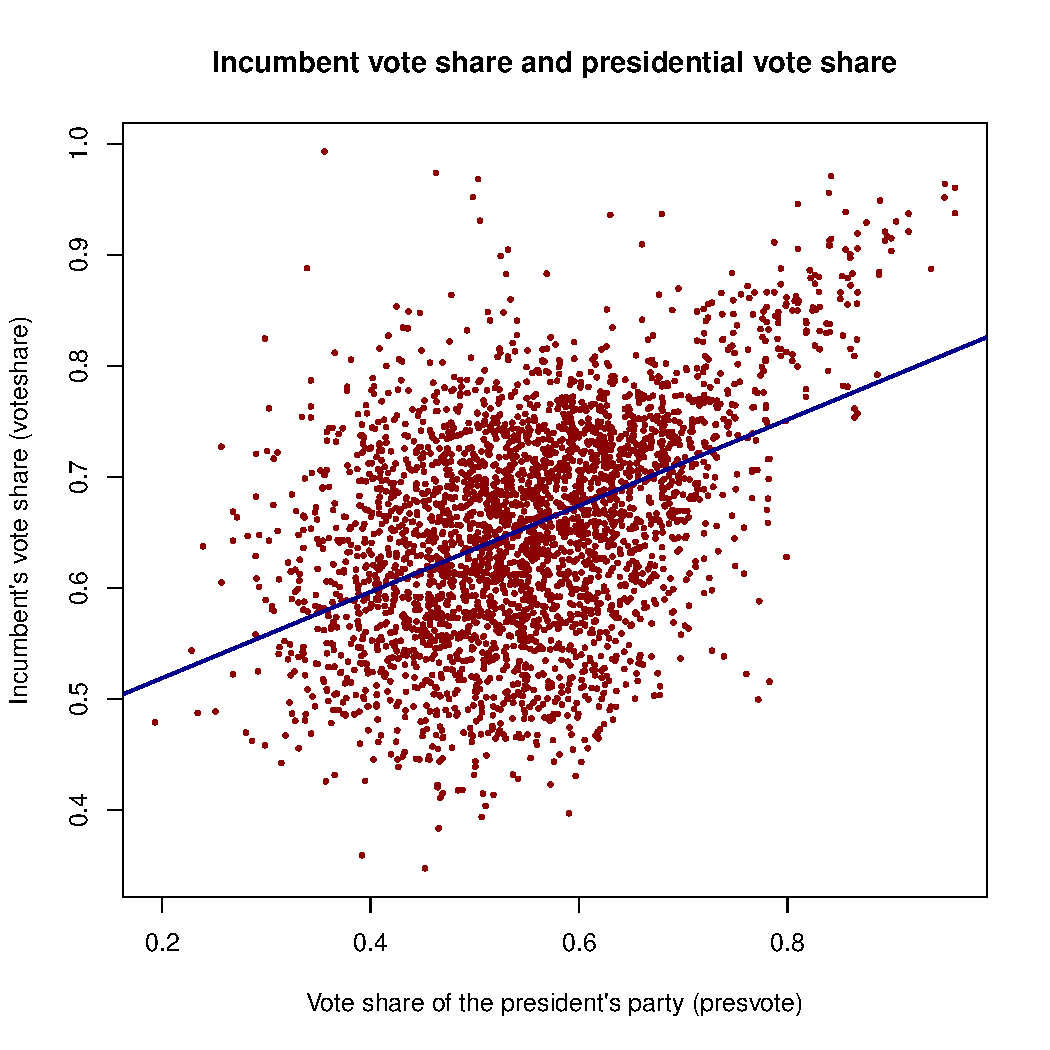
\includegraphics[width=0.7\textwidth]{plot_q3.pdf}
			\caption{Scatterplot of \texttt{voteshare} and \texttt{presvote} with the regression line}
		\end{figure}
		
		\noindent The scatterplot shows a positive relationship: incumbents tend to do better in districts where the presidential candidate of their party also does better.
		
		\item Write the prediction equation.
		
		\[
		\widehat{\texttt{voteshare}}_i = 0.441 + 0.388 \times \texttt{presvote}_i
		\]
	\end{enumerate}
	
	\section*{Question 4}
	\noindent The residuals from part (a) tell us how much of the variation in \texttt{voteshare} is $not$ explained by the difference in spending between incumbent and challenger. The residuals in part (b) tell us how much of the variation in \texttt{presvote} is $not$ explained by the difference in spending between incumbent and challenger in the district.
	\begin{enumerate}
		\item Run a regression where the outcome variable is the residuals from Question 1 and the explanatory variable is the residuals from Question 2.
		
		\noindent To run the regression, I used the \texttt{lm()} function in \texttt{R}, with the residuals from Question 1 (\texttt{resid\_1}) as the outcome variable and the residuals from Question 2 (\texttt{resid\_2}) as the explanatory variable. The results are reported in Table~\ref{tab:regression_q4}.
		
		\lstinputlisting[language=R, firstline=165, lastline=165]{PS03_answersEL.R}
		
		
\begin{table}[H] \centering 
  \caption{Regression of the residuals of Question 1 on the residuals of Question 2} 
  \label{tab:regression_q4} 
\begin{tabular}{@{\extracolsep{5pt}}lc} 
\\[-1.8ex]\hline 
\hline \\[-1.8ex] 
 & \multicolumn{1}{c}{\textit{Dependent variable:}} \\ 
\cline{2-2} 
\\[-1.8ex] & Residuals of Question 1 (resid\_1) \\ 
\hline \\[-1.8ex] 
 Residuals of Question 2 (resid\_2) & 0.257$^{***}$ \\ 
  & (0.012) \\ 
  & \\ 
 Constant & $-$0.000 \\ 
  & (0.001) \\ 
  & \\ 
\hline \\[-1.8ex] 
Observations & 3,193 \\ 
R$^{2}$ & 0.130 \\ 
Adjusted R$^{2}$ & 0.130 \\ 
Residual Std. Error & 0.073 (df = 3191) \\ 
F Statistic & 476.975$^{***}$ (df = 1; 3191) \\ 
\hline 
\hline \\[-1.8ex] 
\textit{Note:}  & \multicolumn{1}{r}{$^{*}$p$<$0.1; $^{**}$p$<$0.05; $^{***}$p$<$0.01} \\ 
\end{tabular} 
\end{table}  

		
		\noindent The intercept is 0 because both sets of residuals have a mean of 0. The slope (0.257) shows the relationship between \texttt{presvote} and \texttt{voteshare} after the effect of \texttt{difflog} has been removed from both variables. It is smaller than the slope in Question 3 (0.388), because part of the relationship between \texttt{presvote} and \texttt{voteshare} was due to their common relationship with \texttt{difflog}. The slope is still statistically significant (p-value $< 0.001$).
		
		\item Make a scatterplot of the two residuals and add the regression line.
		
		\lstinputlisting[language=R, firstline=177, lastline=182]{PS03_answersEL.R}
		
		\begin{figure}[H]
			\centering
			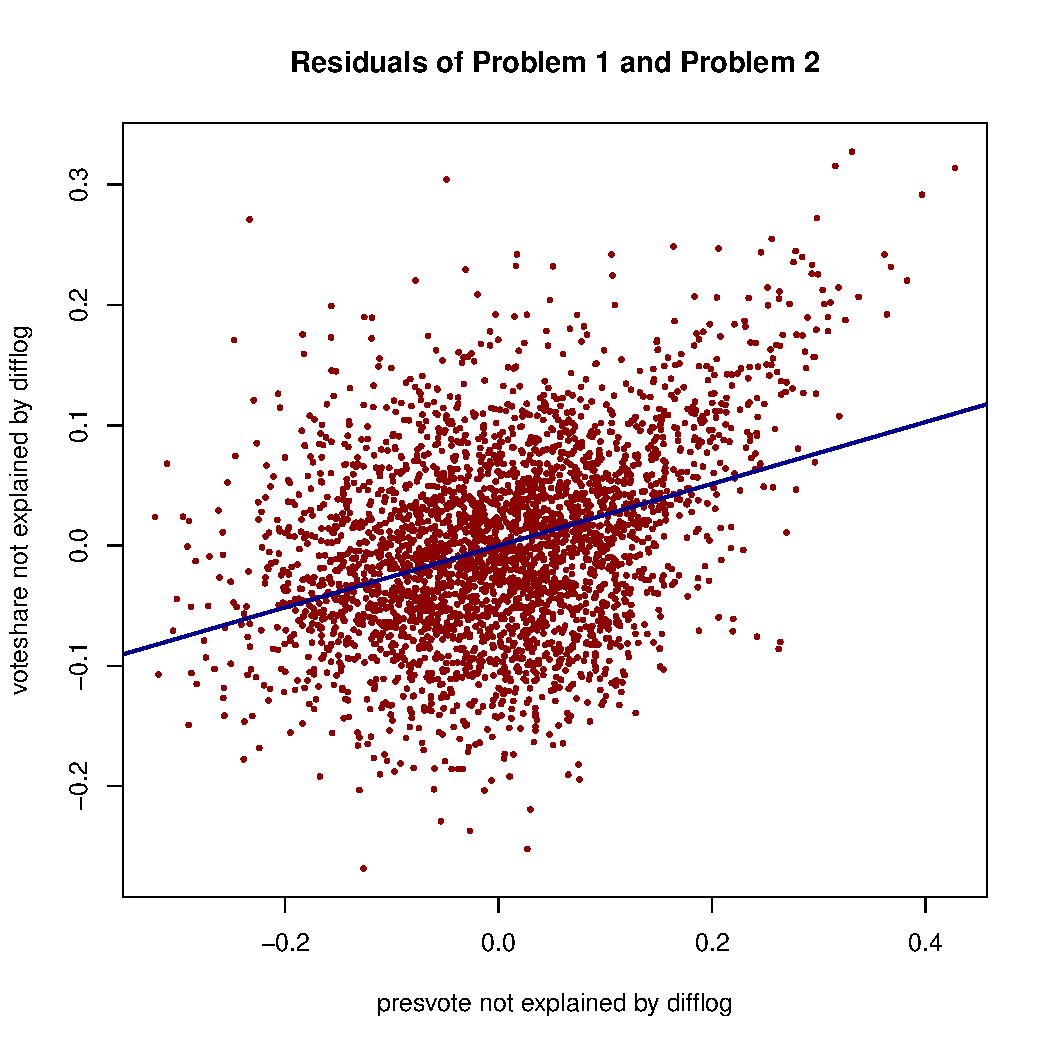
\includegraphics[width=0.7\textwidth]{plot_q4.pdf}
			\caption{Scatterplot of residuals of Question 1 against residuals of Question 2}
		\end{figure}
		
		\noindent The points are centred around $(0, 0)$ and the line goes upward, showing that \texttt{presvote} is still positively related to \texttt{voteshare} once \texttt{difflog} is taken into account.
		
		\item Write the prediction equation.
		
		\[
		\widehat{\texttt{resid\_1}}_i = 0 + 0.257 \times \texttt{resid\_2}_i
		\]
	\end{enumerate}
	
	\section*{Question 5}
	\noindent What if the incumbent's vote share is affected by both the president's popularity and the difference in spending between incumbent and challenger? 
	\begin{enumerate}
		\item Run a regression where the outcome variable is the incumbent's \texttt{voteshare} and the explanatory variables are \texttt{difflog} and \texttt{presvote}.
		
		\noindent To run the regression, I used the \texttt{lm()} function in \texttt{R}, with \texttt{voteshare} as the outcome variable and \texttt{difflog} and \texttt{presvote} as the explanatory variables. The results are reported in Table~\ref{tab:regression_q5}.
		
		\lstinputlisting[language=R, firstline=195, lastline=195]{PS03_answersEL.R}
		
		
\begin{table}[H] \centering 
  \caption{Regression of incumbent's vote share on difference in spending and presidential vote share} 
  \label{tab:regression_q5} 
\begin{tabular}{@{\extracolsep{5pt}}lc} 
\\[-1.8ex]\hline 
\hline \\[-1.8ex] 
 & \multicolumn{1}{c}{\textit{Dependent variable:}} \\ 
\cline{2-2} 
\\[-1.8ex] & Incumbent's vote share (voteshare) \\ 
\hline \\[-1.8ex] 
 Difference in spending (difflog) & 0.036$^{***}$ \\ 
  & (0.001) \\ 
  & \\ 
 Vote share of the president's party (presvote) & 0.257$^{***}$ \\ 
  & (0.012) \\ 
  & \\ 
 Constant & 0.449$^{***}$ \\ 
  & (0.006) \\ 
  & \\ 
\hline \\[-1.8ex] 
Observations & 3,193 \\ 
R$^{2}$ & 0.450 \\ 
Adjusted R$^{2}$ & 0.449 \\ 
Residual Std. Error & 0.073 (df = 3190) \\ 
F Statistic & 1,302.947$^{***}$ (df = 2; 3190) \\ 
\hline 
\hline \\[-1.8ex] 
\textit{Note:}  & \multicolumn{1}{r}{$^{*}$p$<$0.1; $^{**}$p$<$0.05; $^{***}$p$<$0.01} \\ 
\end{tabular} 
\end{table}  

		
		\noindent The intercept (0.449) is the predicted vote share of the incumbent when both explanatory variables are 0, that is, when the incumbent and the challenger spend the same amount and the presidential candidate of the incumbent's party receives no votes in the district. Since \texttt{presvote} is never close to 0 in the data (its minimum is about 0.19), this situation does not exist in practice, so the intercept mainly serves to position the regression line. Holding \texttt{presvote} constant, a one unit increase in \texttt{difflog} is associated with an increase of about 0.036 in the incumbent's vote share. Holding \texttt{difflog} constant, a 1 percentage point increase in \texttt{presvote} is associated with an increase of about 0.26 percentage points in the incumbent's vote share. Both coefficients are statistically significant (p-value $< 0.001$), and together the two variables explain about 45\% of the variation in \texttt{voteshare}.
		
		\item Write the prediction equation.
		
		\[
		\widehat{\texttt{voteshare}}_i = 0.449 + 0.036 \times \texttt{difflog}_i + 0.257 \times \texttt{presvote}_i
		\]
		
		\item What is it in this output that is identical to the output in Question 4? Why do you think this is the case?
		
		\noindent The coefficient of \texttt{presvote} in Question 5 is identical to the slope of \texttt{resid\_2} in Question 4: both are 0.257, with the same standard error (0.012), so the two models also give the same t value and the same p-value.
		
		\noindent This happens because both models measure the same thing, namely the effect of \texttt{presvote} on \texttt{voteshare} after controlling for \texttt{difflog}. In Questions 1 and 2, we removed the effect of \texttt{difflog} from both variables: the residuals from Question 1 are the part of \texttt{voteshare} that is not explained by \texttt{difflog}, and the residuals from Question 2 are the part of \texttt{presvote} that is not explained by \texttt{difflog}. When we regress the first residuals on the second in Question 4, we are left only with the relationship between \texttt{presvote} and \texttt{voteshare} that does not depend on \texttt{difflog}. This is exactly what multiple regression does when it estimates the coefficient of \texttt{presvote} in Question 5, which is interpreted as the effect of \texttt{presvote} holding \texttt{difflog} constant.
		
		\noindent This also explains why the coefficient of \texttt{presvote} (0.257) is smaller than in the simple regression of Question 3 (0.388). Since \texttt{difflog} is related to both \texttt{voteshare} and \texttt{presvote}, the simple regression attributes to \texttt{presvote} part of the variation in \texttt{voteshare} that is actually shared with \texttt{difflog}. If we did not control for \texttt{difflog}, we would therefore overestimate the effect of \texttt{presvote} on the incumbent's vote share.
	\end{enumerate}
	
\end{document}

